\documentclass[a4paper,12pt,oneside,english]{article}

\usepackage{times}  
\usepackage{amsmath}
\usepackage{amssymb}
\usepackage{graphicx}
\usepackage{theorem}
\usepackage[latin1]{inputenc}
\usepackage{latexsym}
\usepackage{url}
\usepackage{babel}
\usepackage{epstopdf}


%Labels



\begin{document}

\section{Inledning}

\section{Method}
Below we present the method of the project.

\subsection{2.1	C\#/.Net and XNA}
The executable files for this project was written the programming language C\# and Microsoft .NET was utilized as a framework. To make graphics easier to display the environment Microsoft XNA was used. 


\subsection{Marching cubes}
Marching cubes is an algorithm for making particles "melt" together and construct a surface or so called "mesh". Developed by Cline and Lorensen in 1987, at the time working for General Electric Company, marching cubes uses 256 cube configurations to represent every way the mesh could cross the cube. Utilizing symmetries can reduce the configurations to 15 unique patterns.

	\begin{figure}[htb]
	\begin{center}
		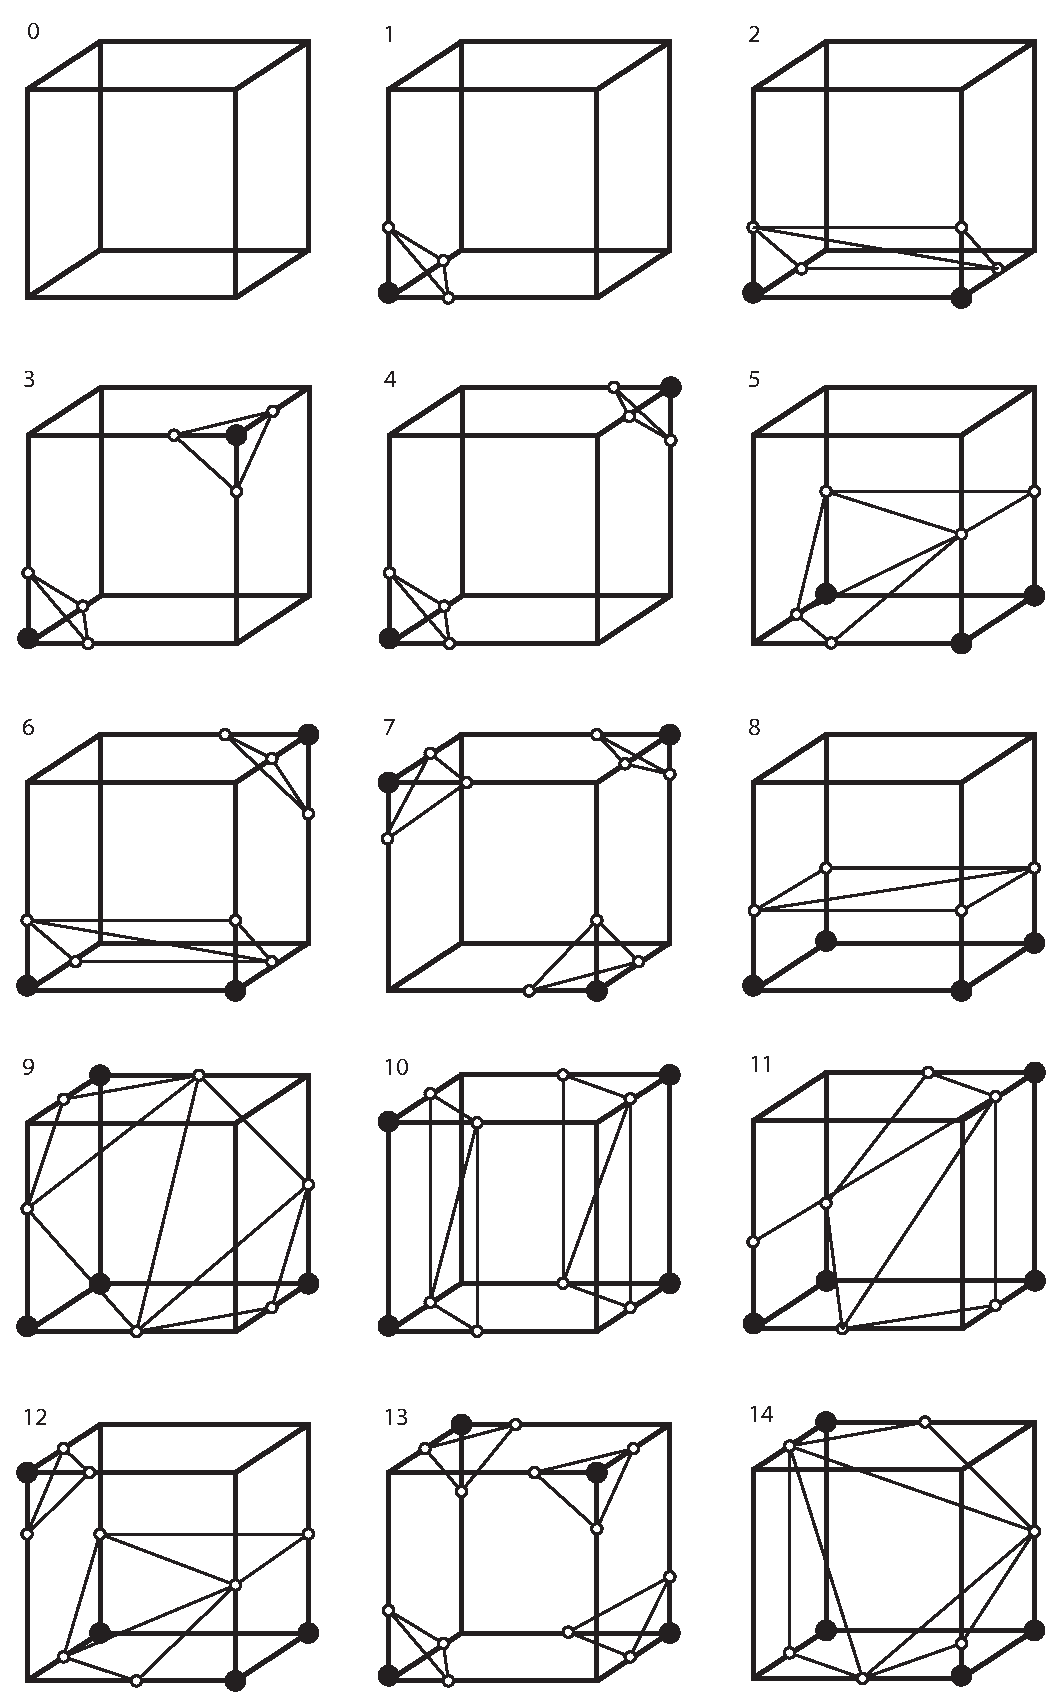
\includegraphics[scale=0.5]{Figures/marching_cubes.eps}
			\caption{Marching}
	\end{center}
		\label{MarchingCubes}
	\end{figure}	\subsection{Partiklar}
	\subsection{Navier Stokes ekvationer}

\section{Usage}
	\subsection{Computer games}
	In computer games of today the player is likely to encounter some sort of fluid being simulated, whether it be water, smoke etcetera. In order to improve rendering speed and visual quality of the simulation, some physical details are sacrificed. To interact with fluids in game the simulation is usually done by graphic card calculations.
	
	\subsection{Movies}
	On the contrary to computer games, where the focus lies in rendering speed, the most important factor of fluid simulations in movies is its visual appearance. Real-time rendering is not necessary in movies, thus enabling heavier calculations, should that be required for the visual appearance.

\section{Systembeskrivning}


	\subsection{System}
The system that we have built is a fluid represented by particles. Different forces act on the particles which causes them to move the way they do. Fluids are materials that are being deformed under forces. They are commonly known to be liquids but fluids are also gases. Our model is capable simulating a gas like substance. However, the focus was mainly on creating a liquid. Normally, a simulation system is described with a bond graph or block diagram. In our case though, because this is a particle based fluid simulation, which requires quite a lot of particles to look like liquid, it is hard.

	\subsection{SPH, Smoothed Particle Hydrodynamics}
	Smoothed Particle Hydrodynamics (SPH), as developed by Lucy and Gingold, is originally a method of simulating astrophysical problems, but is sufficient enough to simulate any kind of fluid. According to SPH, a scalar quantity A is interpolated at location r by a weighted sum of contributions from all particles:
	
	\[
	A_{S}(\textbf{r}) = {\sum_{j}} m_{j} \frac{A_{j}}{\rho_{j}} W(\textbf{r}-\textbf{r}_{j},h)
\]
	
	%\subsection{Model}

	\subsection{Physical history}
	Many people have studied the behavior of fluids for many centuries. One method to describe how fluids behave (describe the motion of substances) is the Navier-Stokes equations, named after Claude-Louis Navier and George Gabriel Stokes. This method is used for this project.

	As seen in the equation below, the physical quantities used are pressure, density and viscosity.
	
	\[
	\rho\left(\frac{\partial v}{\partial t} + v \cdot\nabla v\right) = -\nabla p + \rho g + \mu\nabla^{2}v
\]

	\subsection{Pressure}
		
	\subsection{Density}
	The force caused by the density that affects each particle is calculated as the sum of all forces of the particles within the interaction distance, which is the maximum distance in which a particle can have a neighbor, and outer forces such as gravity.

	For each particle, loop through the particle's neighbors and multiply each neighbors' $W(\textbf{r}-\textbf{r}_{j},h)$.

	\[
	\rho_{S}(\textbf{r}) = {\sum_{j}} m_{j}W(\textbf{r}-\textbf{r}_{j},h)
\]
	
	\subsection{Viscosity}
	Viscosity is caused by friction which converts the particle's kinetic energy to heat.
	The viscosity is calculated by looking at the force in the gradient of the neighbors of each particle.
	
		
	\subsection{Kraftsimulering}
	

\section{L�sningsmetod}
	
(Implementering)
\section{Genomf�ra}
	\subsection{Acceleration}

Kollisionshantering
	Dimensionsf�rlust och idealiserade plan
	Parallellisering
	Sorteringsalgoritmer

Rendering

Resultat

Slutsats
\end{document}